\subsection{Multipath Probing}
%\li: add the two path one flow example
\begin{figure}
\centering
%\begin{minipage}{.45\textwidth}
  \centering
  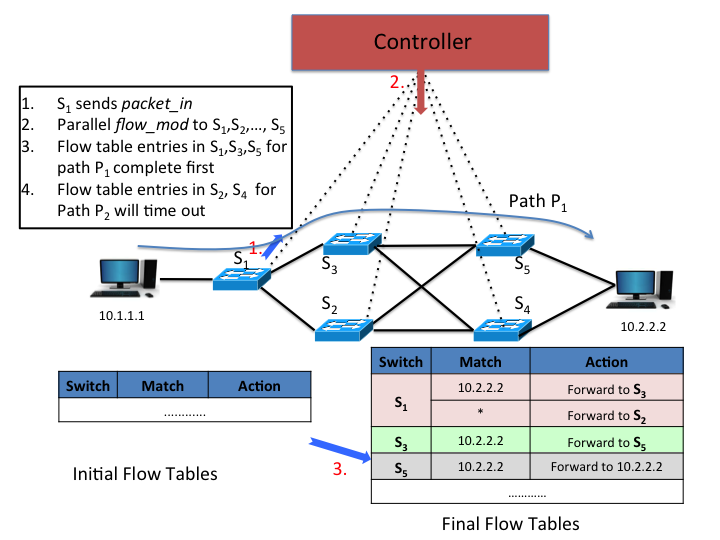
\includegraphics[width=3.5in]{figs/Mazu-mpath.png}
\caption{Exploiting parallel path setup}
\label{fig:mpath}
\end{figure}
%At the lowest level, Broadcom's SDK writes entries to specific addresses in the
%TCAM. If there are multiple entries, the one at the lower address always
%wins. But when you insert a single entry, the Broadcom SDK has no idea whether
%most of the entries you will insert later will be higher or lower
%priority. Nevertheless, it needs to pick an address. Whatever it picks it will
%be wrong for some input pattern. The update rates you see will depend on the
%specific heuristics used for picking addresses -- I do not know the
%specifics. The problem is that after inserting a small percentage of the
%entries, you will want to insert a new one between two existing entries, but
%they will be at adjacent addresses. So you have to make room by doing a
%"shuffle". It's no big deal if you only need to move one entry up or down by one
%address to make room, but as the device fills up you may need  to shuffle a
%large percentage of the entries to make room for the newcomer. Neither is it
%possible to game the system and make a lot of room for future entries because
%you don't know where they will need the room. Again, there are heuristics
%governing shuffles and how aggressively and proactively they are done -- I don't
%know the specifics of what they use. 

As we have seen in Figure x, \flowmod\ delay can be significantly affected by
other switch agent activities such as polling flow statistics.
%$flow\_mod$ time can be very preditable if all of
%them have the same priority. This is because no TCAM rule shuffles are needed.
%However, when rules have different priorities, different addresses are
%picked. Depending on the addresses picked, one may need to make room for new
%entries. Thus, shuffling may happen. \aditya{I don't think we want to use this
%  as a motivation because it contradicts what we are doing for flow engineering,
%  where we assume that the impact of priorities is predictable. why not use
%  pollstats and other uncontrolled activity as motivation??}  
%
To deal with unpredictible delay, we try to setup multiple paths. Data plane packets will
flow as soon as one path completes the setup. 
%\aditya{from here on out, the section was very hard to follow}
First, we illustrate our ideas using a simple example in
Figure~\ref{fig:mpath}. In this five-switch toplogy with switch
$S_1$,$S_2$,$\cdots$, $S_5$, host 10.1.1.1 originates a flow to host
10.2.2.2. Initially all flow tables are empty.
%entry that forward traffic to $S_2$. That is, $S_1$ delegates $packet\_in$
%processing to $S_2$. The reason for the delegation approach is to guard again the
%case that it takes sw1 a long time to install the rules. \emph{Essentially, we create
%two parallel paths even if a flow has a single ingress!} 
When sw1 receives the packet from 10.1.1.1, it will perform
the $packet\_in$ function (step 1). This can be done through our middlebox idea or
directly involve $S_1$'s CPU to generate a $packet\_in$ message and send to
controller. 
%The key point to note is that the $packet\_in$ message will have the
%incoming port information. For our middlebox idea, the incoming port ID can be
%stamped in the IPID field of the first packet before label switch it to the
%middlebox. 

%When the controller receives the $packet\_in$ message with the incoming port
%information, it knows that switch $S_2$ is acting as the delegate of switch
%$S_1$. 
In step 2 shown in the figure, the controller will set parallel
$flow\_mod$ messages to install rules for two paths: (1) path 1 is $S_1$,$S_3$,
$S_5$; (2) path 2 (except ingress) is $S_2$, $S_4$. In order for the controller to know
that $flow\_mod$ has appeared in a switch's hardware flow table, the controller
can send barrier messages to switches. Barrier messages request switch to notify
the controller when all rules before the barrier message is installed (not all
switch implement barrier message or implement it with a 
blocking semantics, i.e. barrier reply message is sent after the rule appears in
TCAM).  %\aditya{the sentence in paranthesis does not parse}

There are two cases. Case 1: suppose the controller
receives the barrier reply messages from all switches in path $P_1$ before path
2's $S_2$ and $S_4$. The controller will send a $packet\_out$ message to switch $S_1$. 
%The controller supplies the complete packet in the message. 
The first packet will be routed
through switch $S_3$ and $S_5$ to the destination. Our middlebox idea nicely
handles the case that multiple packets accumulate before the path setup
completes. Switch $S_2$ and $S_4$'s rule entries for path 2 will be timed out
since no traffic will follow. Case 2: path $P_2$'s $S_2$, $S_4$ comes back
first. Suppose $S_1$ also comes back. Then the controller will modify the rule
entry so that the action will direct traffic to path 2.   
% However, when the entry for 10.2.2.2 appears in $S_1$'s hardware flow
%table. Packets will match this high priority rule. So the flow from 10.1.1.1 to
%10.2.2.2 will experience a path switching. If we pick the two paths with similar
%latency, packet reordering should be easily handled at the destination. After
%the switching, rule entries at sw2 and sw4 will be timed out.

\program{prog:mflow-mpath}
    {Parallel Path Setup for Multiple Flows}
{
//$N$ flows, compute $K$ disjoint paths per flow \\
//$maxNEntries$: maximal additional entries we place in each switch \\
while ($i<K$) \{ \\
\> while ($j<N$) \{ \\
\>\>ComputeDisjointPath($flow_j$, $i$) //prune switches belong to more than \\
\>\>\> $maxNEntries$ paths \\
\>\>    $j = j+1$ \\
\> \} \\    
\> $i=i+1$ \\
}

Now we describe an algorithm that can work with concurrent setups of many
flows and each flow can have $K$ paths. For a target application such as
mobility, each UE demands a path with low data plane latency. Instead of
computing one shortest path (in terms of latency), we compute $K$ disjoint
shortest paths or $K$ paths such that each switch belongs to at most $L$ paths,
$L<K$. For simplicity, we consider the former. This problem is NP-hard. We can
take any known good approximation algorithm. We can concurrently setup these
$K$ paths in parallel as in our example. 

For joint solution of multiple flows, we will impose a constraint that no
switch should handle more than $MaxNEntries$ number of $flow\_mod$.  For
fairness, we compute one path for all flows before computing the second
joint path for all flow and so on.  The algorithm is shown in
Figure~\ref{prog:mflow-mpath}. 

%\li{add the algorithm pseudo code}

\iffalse
For mobility, we can compute K-paths per flow or jointly. (1) For per flow, lets
use K shortest paths (i.e. ECMP). These K paths should be disjoint or share
minimal number of switches. Lets use disjoint paths. (2) For joint solution of
multiple flows, we will have the same MaxNEntries constraint per switch. For
fairness, you can compute one path for all flows before computing the second
joint path for all flow, etc.  


Even while I was at Broadcom I had little visibility into how the switch guys'
software handled their TCAM. Now that I'm outside I have zero visibility (I work
on search, not on network infrastructure at Google). But I have a broad
explanation of what you see that I am pretty confident is correct. 
 
The API allows you to associate priorities with rules/entries. The API does not
let you tell the hardware how many lower priority or higher priority rules you
will insert in the future. Nor is this easy to figure out, so even if there were
such API, it would be hard to use. But this is exactly what the software would
need in order to ensure fast updates. A more realistic alternative API would be
to give all the entries at once - I don't know whether such a batch API is
available. 

At the lowest level, Broadcom's SDK writes entries to specific addresses in the
TCAM. If there are multiple entries, the one at the lower address always
wins. But when you insert a single entry, the Broadcom SDK has no idea whether
most of the entries you will insert later will be higher or lower
priority. Nevertheless, it needs to pick an address. Whatever it picks it will
be wrong for some input pattern. The update rates you see will depend on the
specific heuristics used for picking addresses -- I do not know the
specifics. The problem is that after inserting a small percentage of the
entries, you will want to insert a new one between two existing entries, but
they will be at adjacent addresses. So you have to make room by doing a
"shuffle". It's no big deal if you only need to move one entry up or down by one
address to make room, but as the device fills up you may need  to shuffle a
large percentage of the entries to make room for the newcomer. Neither is it
possible to game the system and make a lot of room for future entries because
you don't know where they will need the room. Again, there are heuristics
governing shuffles and how aggressively and proactively they are done -- I don't
know the specifics of what they use. 

One common property of all these TCAM shuffle algorithms is that they work
spectacularly well when entries have the same priority. Shuffles are not
needed. The Broadcom SDK is allowed to write the new entries to any available
TCAM address. 

Please let me know if anything you see contradicts this explanation - there may
be more going on, but usually the shuffles are the big update rate killer. 

Cheers,

Cristi



On Tue, Jan 21, 2014 at 12:59 PM, Aditya Akella <akella@cs.wisc.edu> wrote:
Hi Cristi,

One other question for you that has really been bugging us and we simple can't figure out what's going on. We did a bunch of experiments where we see bizarre and inconsistent results.

Expt 1: We conducted an experiment where we installed a burst of rules of size B of a certain priority pattern P. We measure total latency to install the rules:

1. B --> increasing priority: we see latencies really shoot up, with the burst taking almost 30s to install. This makes sense as perhaps each incoming higher priority rule is causing TCAM rearrangement (?)
2. B --> decreasing priority: we see high latencies too, over 20s to install. We did not expect this as we were hoping the latencies would be the same as B --> same priority.

Any thoughts on what may be going on? So we thought something weird is happening with low/high priorities, so we decided to run a bunch of experiments that played with the pattern of priorities. Here are a couple:

Expt 2: We installed ~700 each of alternating high and low priorities. We saw all rules with the higher priority were installed first (within ~1.5s in all) after which the low priority rules started to get inserted, which kind of makes sense except that the  low latency rule installation completed after 20s or more!

But:

Expt 3: If instead of sending the burst of about 700 above, we first sent 350 high priority rules, and then send a burst of 350 low priority rules after the first batch was installed, then the completion time of the latter is far far lower than what we see in Expt 2.

What on earth is going on? Can you shed some light in general on how Broadcom handles priorities? Is there some obvious issue we are missing out on?

\fi
